%% ----------------------------------------------------------------
%% Thesis.tex -- MAIN FILE (the one that you compile with LaTeX)
%% ---------------------------------------------------------------- 
%%%%%%%%%%%%%%%%%%%%%%%%%%%%%%%%%%%%%%%%%%%%%%%%%%%%%%%%%%%%%%%%%%%%%%%%%%%%%%%%
%%%%%%%%%%%%%%%%%%%%%%%%%%%%%%%%%%%% USAGE %%%%%%%%%%%%%%%%%%%%%%%%%%%%%%%%%%%%%
% NOTES:
%  - This document is a modified thesis document for use at UNR.
%  - It abides by the style required by the department and makes it easy to
%    write a thesis document. Please read through comments to understand how to
%    use this document. There are several steps involved. And there is a word
%    document that is required to build the document fully.
%  - A MakeFile was provided as well to help build the document. You can use
%    to build the document into a PDF format.
%  - A pdfshrink.sh file is also provided to help shrink the final thesis
%    document to email to others and submit. This is a very useful utility as it
%    can shrink a 50MB pdf down to potentially 3MB. This is very useful!!
%  - Many folder are provided as well for structure. 
%    - The [images] folder is where images should go. If you place an image in
%      that folder you should not need to supply an extension of directory when
%      including graphics into your document.
%  - DO NOT
%    - Adjust any of the spacing or margins in this document. This is the most
%      difficult aspect of the thesis setup.
%  - ENJOY!!
%  - IF YOU HAVE QUESTIONS:
%    - CONTACT:
%      - fraser@nevada.unr.edu
%      - Luke Fraser
%%%%%%%%%%%%%%%%%%%%%%%%%%%%%%%%%%%%%%%%%%%%%%%%%%%%%%%%%%%%%%%%%%%%%%%%%%%%%%%%
%%%%%%%%%%%%%%%%%%%%%%%%%%%%%%%%%%%%%%%%%%%%%%%%%%%%%%%%%%%%%%%%%%%%%%%%%%%%%%%%

% Set up the document
\documentclass[letterpaper, 12pt, oneside]{Thesis}
\usepackage[square, numbers, comma, sort&compress]{natbib}

\usepackage{verbatim}  % Needed for the "comment" environment to make LaTeX comments
\usepackage{vector}  % Allows "\bvec{}" and "\buvec{}" for "blackboard" style bold vectors in maths
\usepackage{algorithm}
\usepackage{algorithmic}
\usepackage{subcaption}
\usepackage{moreverb,url}
\usepackage{pdfpages}

%%%%%%%%%%%%%%%%%%%%%%%%%%%%%%%%%%%%%%%%%%%%%%%%%%%%%%%%%%%%%%%%%%%%%%%%%%%%%%%%
%%%%%%%%%%%%%%%%%%%%%%%%%%%%%%%%%% DUMMY TEXT %%%%%%%%%%%%%%%%%%%%%%%%%%%%%%%%%%
% NOTES: This is not needed for the thesis it can be removed. It is only for the
%        dummy text in the document.

\usepackage[english]{babel}
\usepackage{blindtext}
%%%%%%%%%%%%%%%%%%%%%%%%%%%%%%%%%%%%%%%%%%%%%%%%%%%%%%%%%%%%%%%%%%%%%%%%%%%%%%%%

\DeclareGraphicsExtensions{.pdf,.jpeg,.png,.jpg, .eps}
\graphicspath{{images/}}      
\hypersetup{urlcolor=black, colorlinks=true}  % Colours hyperlinks in blue, but this can be distracting if there are many links.

%% ----------------------------------------------------------------
\begin{document}
\fancyhead[R]{}  % Clears all page headers and footers
\rhead{\thepage}  % Sets the right side header to show the page number
\lhead{}
\frontmatter      % Begin Roman style (i, ii, iii, iv...) page numbering

% Set up the Title Page
\title  {A Hierarchical Control Architecture for Robust and Adaptive Robot Control}
%%%%%%%%%%%%%%%%%%%%%%%%%%%%%%%%%%%%%%%%%%%%%%%%%%%%%%%%%%%%%%%%%%%%%%%%%%%%%%%%
%%%%%%%%%%%%%%%%%%%%%%%%%%%%%%%%%%%% AUTHOR %%%%%%%%%%%%%%%%%%%%%%%%%%%%%%%%%%%%
%%%%%%%%%%%%%%%%%%%%%%%%%%%%%%%%%%%%%%%%%%%%%%%%%%%%%%%%%%%%%%%%%%%%%%%%%%%%%%%%
% NOTES: This is the place the the author of the paper is put
\authors{\texorpdfstring
  {\href{Luke.Fraser.A@gmail.com}{Luke Fraser}}
  {Luke Fraser}
}
%%%%%%%%%%%%%%%%%%%%%%%%%%%%%%%%%%%%%%%%%%%%%%%%%%%%%%%%%%%%%%%%%%%%%%%%%%%%%%%%
%%%%%%%%%%%%%%%%%%%%%%%%%%%%%%%%%%%%%%%%%%%%%%%%%%%%%%%%%%%%%%%%%%%%%%%%%%%%%%%%

\addresses  {\groupname\\\deptname\\\univname}  % Do not change this here, instead these must be set in the "Thesis.cls" file, please look through it instead
\date       {\today}
\subject    {}
\keywords   {}
\newgeometry{left=1in, right=1in, top=1in, bottom=1.25in}

%%%%%%%%%%%%%%%%%%%%%%%%%%%%%%%%%%%%%%%%%%%%%%%%%%%%%%%%%%%%%%%%%%%%%%%%%%%%%%%%
%%%%%%%%%%%%%%%%%%%%%%%%%%%% TITLE PAGE PARAMETERS %%%%%%%%%%%%%%%%%%%%%%%%%%%%%
%%%%%%%%%%%%%%%%%%%%%%%%%%%%%%%%%%%%%%%%%%%%%%%%%%%%%%%%%%%%%%%%%%%%%%%%%%%%%%%%
% NOTES: These are the main title paper parameters that need to be edited to
%        supply the the UNR specific title information
\UNIVERSITY{University of Nevada, Reno}
\STUDENT   {Luke A. Fraser}
\ADVISOR   {Dr. Monica Nicolescu/Thesis Advisor}
%%%%%%%%%%%%%%%%%%%%%%%%%%%%%%%%%%%%%%%%%%%%%%%%%%%%%%%%%%%%%%%%%%%%%%%%%%%%%%%%
%%%%%%%%%%%%%%%%%%%%%%%%%%%%%%%%%%%%%%%%%%%%%%%%%%%%%%%%%%%%%%%%%%%%%%%%%%%%%%%%

\maketitle

%%%%%%%%%%%%%%%%%%%%%%%%%%%%%%%%%%%%%%%%%%%%%%%%%%%%%%%%%%%%%%%%%%%%%%%%%%%%%%%%
%%%%%%%%%%%%%%%%%%%%%%%%%%%%%%%% COMMITTEE FORM %%%%%%%%%%%%%%%%%%%%%%%%%%%%%%%%
% NOTES: You will need to generate this pdf document from the .docx word
%        doc found in the main folder. This can also be openned in
%        OpenOffice/LibreOffice. Please use the one provided as there is an
%        error in the one found online. Unless the document changes this will
%        provide you an acceptable alternative to the windows file.
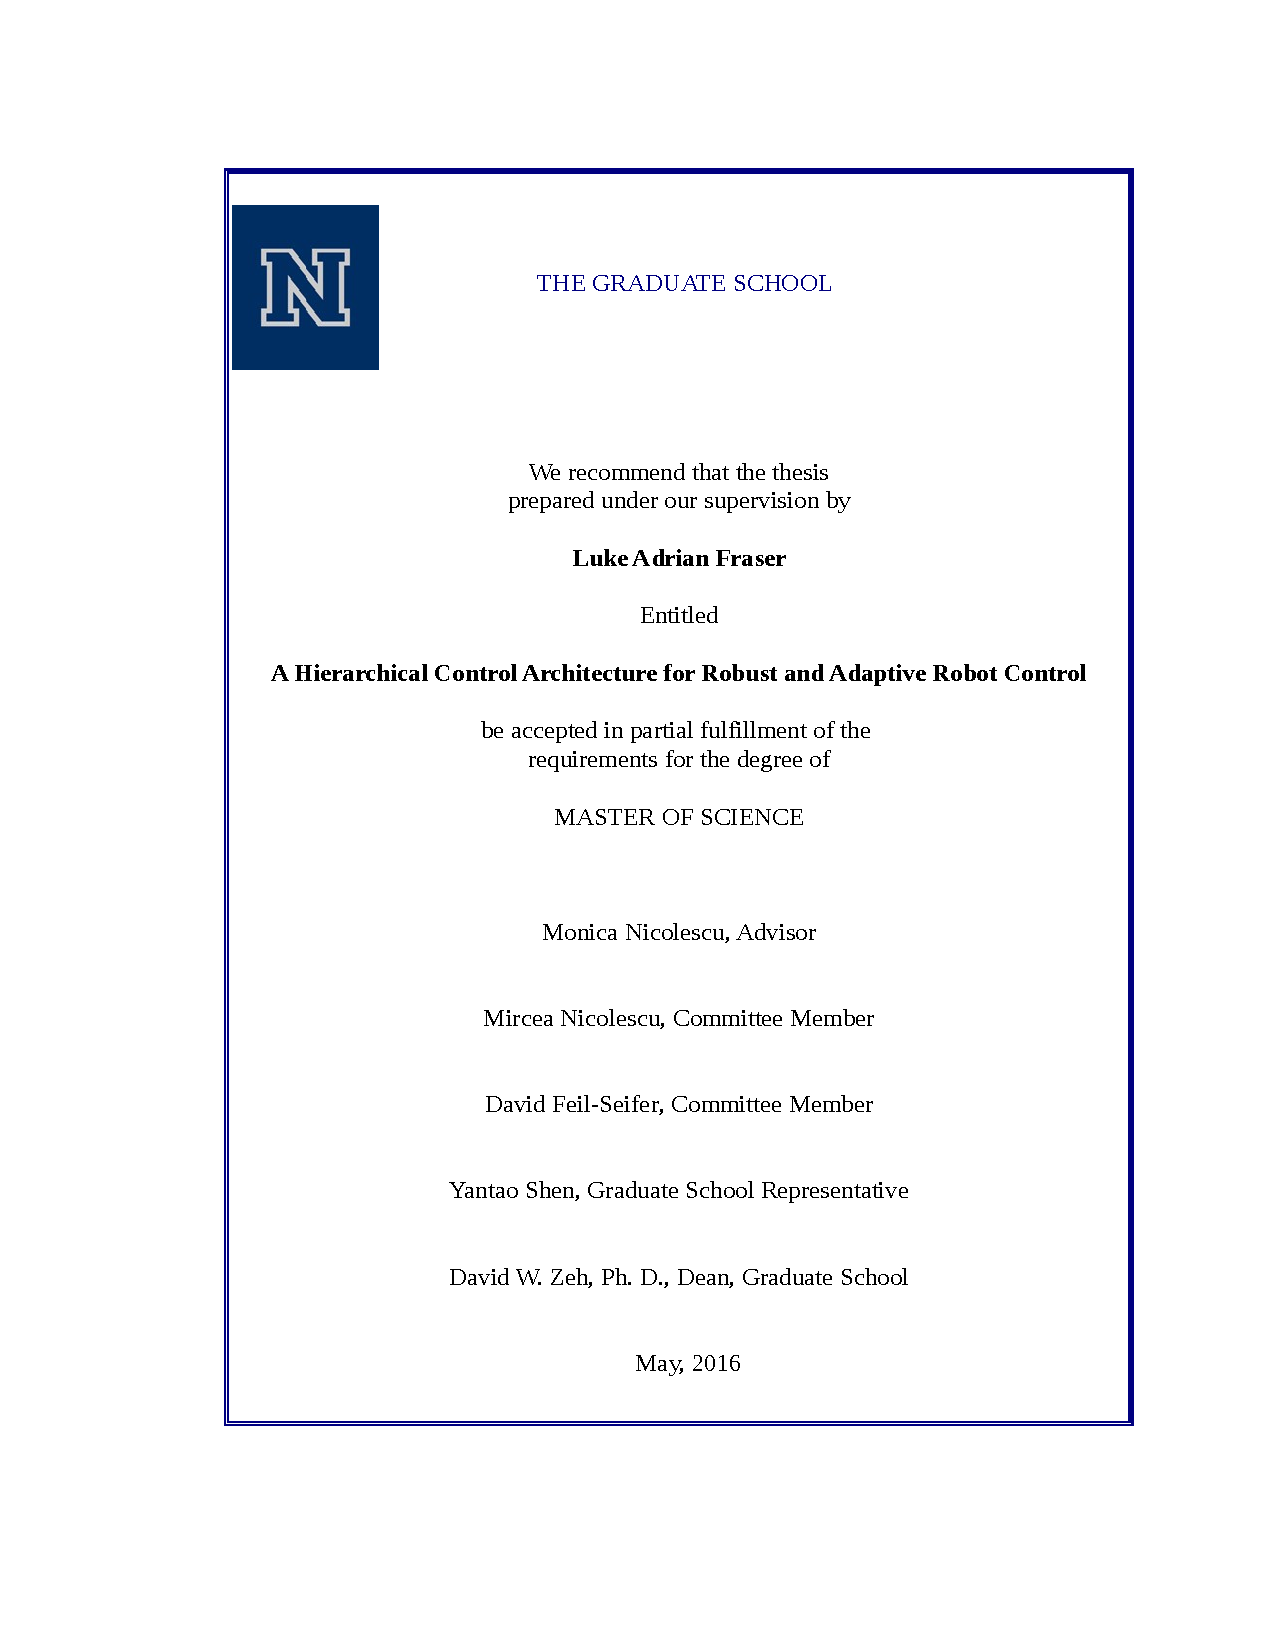
\includepdf{committeeform.pdf}
%%%%%%%%%%%%%%%%%%%%%%%%%%%%%%%%%%%%%%%%%%%%%%%%%%%%%%%%%%%%%%%%%%%%%%%%%%%%%%%%
%%%%%%%%%%%%%%%%%%%%%%%%%%%%%%%%%%%%%%%%%%%%%%%%%%%%%%%%%%%%%%%%%%%%%%%%%%%%%%%%

\newgeometry{left=1.5in, right=1in, top=1in, bottom=1.25in}
\fancypagestyle{plain}{%
  \fancyhf{}
  \renewcommand{\headrulewidth}{0pt}
  \fancyhead[R]{\thepage}
  \fancyhead[C]{}
}

\setstretch{2}  % It is better to have smaller font and larger line spacing than the other way round

% Define the page headers using the FancyHdr package and set up for one-sided printing
% \fancyhead[R]{}  % Clears all page headers and footers
\rhead{\thepage}  % Sets the right side header to show the page number
\lhead{}  % Clears the left side page header

%\pagestyle{fancy}  % Finally, use the "fancy" page style to implement the FancyHdr headers

%% ----------------------------------------------------------------
% Declaration Page required for the Thesis, your institution may give you a different text to place here
% \Declaration{

% \addtocontents{toc}{\vspace{1em}}  % Add a gap in the Contents, for aesthetics

% I, AUTHOR NAME, declare that this thesis titled, `THESIS TITLE' and the work presented in it are my own. I confirm that:

% \begin{itemize} 
% \item[\tiny{$\blacksquare$}] This work was done wholly or mainly while in candidature for a research degree at this University.
 
% \item[\tiny{$\blacksquare$}] Where any part of this thesis has previously been submitted for a degree or any other qualification at this University or any other institution, this has been clearly stated.
 
% \item[\tiny{$\blacksquare$}] Where I have consulted the published work of others, this is always clearly attributed.
 
% \item[\tiny{$\blacksquare$}] Where I have quoted from the work of others, the source is always given. With the exception of such quotations, this thesis is entirely my own work.
 
% \item[\tiny{$\blacksquare$}] I have acknowledged all main sources of help.
 
% \item[\tiny{$\blacksquare$}] Where the thesis is based on work done by myself jointly with others, I have made clear exactly what was done by others and what I have contributed myself.
% \\
% \end{itemize}
 
 
% Signed:\\
% \rule[1em]{25em}{0.5pt}  % This prints a line for the signature
 
% Date:\\
% \rule[1em]{25em}{0.5pt}  % This prints a line to write the date
% }
% \clearpage  % Declaration ended, now start a new page

%% ----------------------------------------------------------------
% The "Funny Quote Page"
\pagestyle{empty}  % No headers or footers for the following pages

% \null\vfill
% % Now comes the "Funny Quote", written in italics
% % \textit{``Write a funny quote here.''}

% % \begin{flushright}
% % If the quote is taken from someone, their name goes here
% % \end{flushright}

% \vfill\vfill\vfill\vfill\vfill\vfill\null
% \clearpage  % Funny Quote page ended, start a new page
%% ----------------------------------------------------------------
\setcounter{page}{1}
% The Abstract Page
\addtotoc{Abstract}  % Add the "Abstract" page entry to the Contents
\abstract{
\blindtext
}

\clearpage  % Abstract ended, start a new page
%% ----------------------------------------------------------------

\setstretch{2}  % Reset the line-spacing to 1.3 for body text (if it has changed)

% The Acknowledgements page, for thanking everyone
\acknowledgements{
\addtocontents{toc}{\vspace{1em}}  % Add a gap in the Contents, for aesthetics
\blindtext[2]
}

\clearpage  % End of the Acknowledgements
%% ----------------------------------------------------------------

% \pagestyle{fancy}  %The page style headers have been "empty" all this time, now use the "fancy" headers as defined before to bring them back


%% ----------------------------------------------------------------
\lhead{\emph{Contents}}  % Set the left side page header to "Contents"
\tableofcontents  % Write out the Table of Contents

%% ----------------------------------------------------------------
\lhead{\emph{List of Figures}}  % Set the left side page header to "List if Figures"
\listoffigures  % Write out the List of Figures

%% ----------------------------------------------------------------
% \lhead{\emph{List of Tables}}  % Set the left side page header to "List of Tables"
% \listoftables  % Write out the List of Tables

%% ----------------------------------------------------------------
\setstretch{2}  % Set the line spacing to 1.5, this makes the following tables easier to read
% \clearpage  % Start a new page
% \lhead{\emph{Abbreviations}}  % Set the left side page header to "Abbreviations"
% \listofsymbols{ll}  % Include a list of Abbreviations (a table of two columns)
% {
% % \textbf{Acronym} & \textbf{W}hat (it) \textbf{S}tands \textbf{F}or \\
% \textbf{LAH} & \textbf{L}ist \textbf{A}bbreviations \textbf{H}ere \\

% }

%% ----------------------------------------------------------------
% \clearpage  % Start a new page
% \lhead{\emph{Physical Constants}}  % Set the left side page header to "Physical Constants"
% \listofconstants{lrcl}  % Include a list of Physical Constants (a four column table)
% {
% % Constant Name & Symbol & = & Constant Value (with units) \\
% Speed of Light & $c$ & $=$ & $2.997\ 924\ 58\times10^{8}\ \mbox{ms}^{-\mbox{s}}$ (exact)\\

% }

%% ----------------------------------------------------------------
% \clearpage  %Start a new page
% \lhead{\emph{Symbols}}  % Set the left side page header to "Symbols"
% \listofnomenclature{lll}  % Include a list of Symbols (a three column table)
% {
% % symbol & name & unit \\
% $a$ & distance & m \\
% $P$ & power & W (Js$^{-1}$) \\
% & & \\ % Gap to separate the Roman symbols from the Greek
% $\omega$ & angular frequency & rads$^{-1}$ \\
% }
%% ----------------------------------------------------------------
% End of the pre-able, contents and lists of things
% Begin the Dedication page

\setstretch{2.0}  % Return the line spacing back to 1.3

% \pagestyle{empty}  % Page style needs to be empty for this page
% \dedicatory{For/Dedicated to/To my\ldots}

% \addtocontents{toc}{\vspace{2em}}  % Add a gap in the Contents, for aesthetics


%% ----------------------------------------------------------------
\mainmatter	  % Begin normal, numeric (1,2,3...) page numbering
\pagestyle{fancy}  % Return the page headers back to the "fancy" style
      \renewcommand{\headrulewidth}{0pt}
\fancyhead[R]{\thepage}  % Clears all page headers and footers
\rhead{\thepage}  % Sets the right side header to show the page number
\lhead{}  % Clears the left side page header
% Include the chapters of the thesis, as separate files
% Just uncomment the lines as you write the chapters

%%%%%%%%%%%%%%%%%%%%%%%%%%%%%%%%%%%%%%%%%%%%%%%%%%%%%%%%%%%%%%%%%%%%%%%%%%%%%%%%
%%%%%%%%%%%%%%%%%%%%%%%%%%%%%%%%%%% CHAPTERS %%%%%%%%%%%%%%%%%%%%%%%%%%%%%%%%%%%
%%%%%%%%%%%%%%%%%%%%%%%%%%%%%%%%%%%%%%%%%%%%%%%%%%%%%%%%%%%%%%%%%%%%%%%%%%%%%%%%
% NOTES: This is where the main content of your thesis is written. You create
%        a new file for every chapter that you write. This isn't mandatory, but
%        it keeps the thesis clean and easy to edit.
\chapter{Introduction}

\blindtext
\blinditemize
\blinddescription \cite{Garcia2008}
\section{Summary}
\blindtext
 % Introduction

\chapter{Related Works}
\label{relatedWork}
\blindtext[2]

\blinddescription

\blindmathtrue

\blindtext

\section{Summary}
\blindtext % Background Theory 

\chapter{Proposed Architecture}
\label{architecture}
\blindtext[3]


\begin{figure}
\centering
  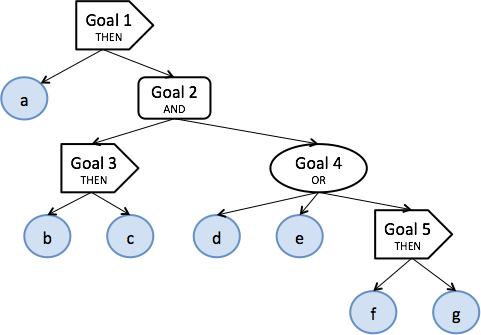
\includegraphics[width=11cm]{task_img}
\caption{Representation of task: a {\bf THEN} ((b {\bf THEN} c) {\bf AND} (d {\bf OR} e {\bf OR} (f {\bf THEN} g))).}
\label{fig:task_representation}
\end{figure}

\blindtext[3]

\section{Update Loop}
\label{sec:updateloop}
\begin{algorithm}
\caption{Behavior update loop}
\label{alg:update}
\begin{algorithmic}[1]
\IF {$Not~Done$}
  \IF {$Is~Active$}
    \IF {$Preconditions$}
      \IF {$BEHAVIOR~NODE$}
      \STATE $Activate:$
        \STATE $~~~Mutex Acquired \Rightarrow state \leftarrow running$
      \ELSIF {$GOAL~NODE$}
        \STATE $Activate:$
          \STATE $~~~state \leftarrow done$
      \ENDIF
    \ELSE
      \STATE $SpreadActivation$
    \ENDIF
    \STATE \emph{ActivationFalloff} $\Rightarrow \alpha ~*$ \emph{activation\_level}  
  \ENDIF
\ENDIF
\end{algorithmic}
\label{update-loop}
\end{algorithm}

\subsection{Activation Potential Spreading}
\blindtext
%%%%%%%%%%%%%%%%%%%%%%%%%%%%%%%%%%%%%%%%%%%%%%%%%%%%%%%%%%%%%%%%%%%%%%%%%%%%%%%%
\begin{figure}
\centering
  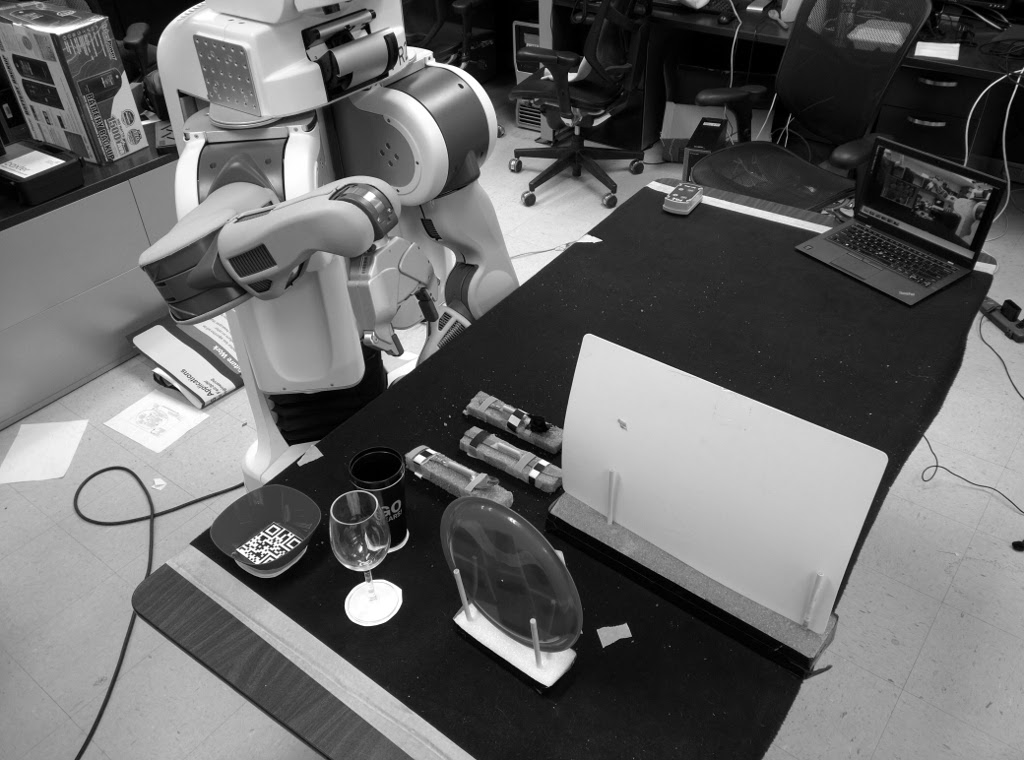
\includegraphics[width=\textwidth]{bw_task_environment}
\caption{Experimental setup.}
\label{fig:setup}       % Give a unique label
\end{figure}
%%%%%%%%%%%%%%%%%%%%%%%%%%%%%%%%%%%%%%%%%%%%%%%%%%%%%%%%%%%%%%%%%%%%%%%%%%%%%%%%
%%%%%%%%%%%%%%%%%%%%%%%%%%%%%%%%%%%%%%%%%%%%%%%%%%%%%%%%%%%%%%%%%%%%%%%%%%%%%%%%

\section{Summary}
\blindtext % Experimental Setup

\chapter{Experimental Evaluation}
\label{evaluation}

\blindtext[2] % Experiment 1

% \input{Chapters/Chapter5} % Experiment 2

\chapter{Conclusion \& Future Work}
\label{conclusion}
\blindtext[2] % Results and Discussion

%\input{Chapters/Chapter7} % Conclusion
%%%%%%%%%%%%%%%%%%%%%%%%%%%%%%%%%%%%%%%%%%%%%%%%%%%%%%%%%%%%%%%%%%%%%%%%%%%%%%%%
%%%%%%%%%%%%%%%%%%%%%%%%%%%%%%%%%%%%%%%%%%%%%%%%%%%%%%%%%%%%%%%%%%%%%%%%%%%%%%%%
%% ----------------------------------------------------------------
% Now begin the Appendices, including them as separate files

% \addtocontents{toc}{\vspace{2em}} % Add a gap in the Contents, for aesthetics

% \appendix % Cue to tell LaTeX that the following 'chapters' are Appendices

% \input{Appendices/AppendixA}	% Appendix Title

%\input{Appendices/AppendixB} % Appendix Title

%\input{Appendices/AppendixC} % Appendix Title

% \addtocontents{toc}{\vspace{2em}}  % Add a gap in the Contents, for aesthetics
\backmatter

%% ----------------------------------------------------------------
\label{Bibliography}
\lhead{\emph{Bibliography}}  % Change the left side page header to "Bibliography"
\bibliographystyle{unsrtnat}  % Use the "unsrtnat" BibTeX style for formatting the Bibliography
\bibliography{refs/master}  % The references (bibliography) information are stored in the file named "Bibliography.bib"

\end{document}  % The End
%% ----------------------------------------------------------------